% Note: the document is written in LaTeX, hence the commands and macros in the manuscript.
% If you’re familiar with LaTeX, don’t hesitate to modify the commands, otherwise treat this document as a normal word document.

\documentclass[essd, manuscript]{copernicus}
\graphicspath{{../figures/paper/}}


\begin{document}

\title{Eutrophication climatologies for the European Seas}

\Author[1]{Charles}{Troupin}
\Author[1]{Alexander}{Barth}
\Author[2]{Karin}{Wesslander}
\Author[3]{Julie}{Gatti}
\Author[3]{Amandine}{Thomas}
\Author[3]{Erwann}{Quimpert}
\Author[5]{Jonas}{Koefoed Romer}
\Author[5]{Martin}{Mork Larsen}
\Author[6]{Luminita}{Buga}
\Author[6]{George}{Sarbu}
\Author[7]{Sissy}{Iona}
\Author[7]{Marilena}{Tsompanou}
\Author[8]{Ann Kristin}{Ostrem}
\Author[4]{Maria Eugenia}{Molina Jack}
\Author[4]{Marina}{Lipizer}
\Author[9]{Dick}{Schaap}
\Author[4]{Alessandra}{Giorgetti}


\affil[1]{University of Liège, FOCUS Research Unit, GeoHydrodynamics and Environment Research group (GHER), Allée du 6-Août, 17, 4000 Liège 1, Belgium} 
\affil[2]{Swedish Meteorological and Hydrological Institute Oceanographic Laboratory 2020-01-17 Dnr S/Gbg-2020-1 Address Sven Källfelts Gata 15 426 71 Västra Frölunda}
\affil[3]{French Institute for Ocean Science (IFREMER), 1625 Route de Sainte-Anne, 29280 Plouzané, France}
\affil[5]{Aarhus University, Department of Bioscience - Marine Diversity and Experimental Ecology, Frederiksborgvej 399 building 7411, B1.21, 4000 Roskilde, Denmark}
\affil[7]{Hellenic National Oceanographic Data Centre, 46,7 km Athens Sounio, Mavro Lithari P.O. BOX 712 19013 Anavissos, Attica, Greece}
\affil[6]{National Institute for Marine Research and Development “Grigore Antipa”. Location. B-dul Mamaia Nr. 300, Romina}
\affil[8]{Institute of Marine Research, P.O box 1870 Nordnes NO-5817 Bergen, Norway}
\affil[4]{Istituto Nazionale di Oceanografia e di Geofisica Sperimentale - OGS Borgo Grotta Gigante 42/C, 34010 Sgonico (TS), Italy}
\affil[9]{MARIS BV, Gildeweg 7 A BD Nootdorp, The Netherlands} %0000-0001-6562-068X


%% If authors contributed equally, please mark the respective author names with an asterisk, e.g. "\Author[2,*]{Anton}{Smith}" and "\Author[3,*]{Bradley}{Miller}" and add a further affiliation: "\affil[*]{These authors contributed equally to this work.}".


\correspondence{Charles Troupin (ctroupin@uliege.be)}

\runningtitle{Eutrophication climatologies for the European Seas}

\runningauthor{Troupin et al.}


\received{}
\pubdiscuss{} %% only important for two-stage journals
\revised{}
\accepted{}
\published{}

%% These dates will be inserted by Copernicus Publications during the typesetting process.


\firstpage{1}

\maketitle



\begin{abstract}
TEXT
\end{abstract}


\introduction  %% \introduction[modified heading if necessary]
TEXT

The rest of the manuscript is organised as follows: first we describe the in situ observations used for the creation of the gridded products, since they already constitute a useful product; then we present the gridded technique, DIVAnd, applied to the obsertations; finally we describe the final product (climatologies). 


\section{In situ datasets\label{sec:insitu}}

- Describe EMODnet \citep{MartinMiguez2019} 
- Describe EMODnet Chemistry \citep{Giorgetti2018}

Two main types of data are considered: the profiles and the time series. They are processed separately but then used together for the production of the climatologies. Six variables (concentrations) were considered (Sec.~ref{}): ammonium, chlorophyll-a, dissolved oxygen, dissolved inorganic nitrogen, phosphate and silicate.


\begin{figure}[t]
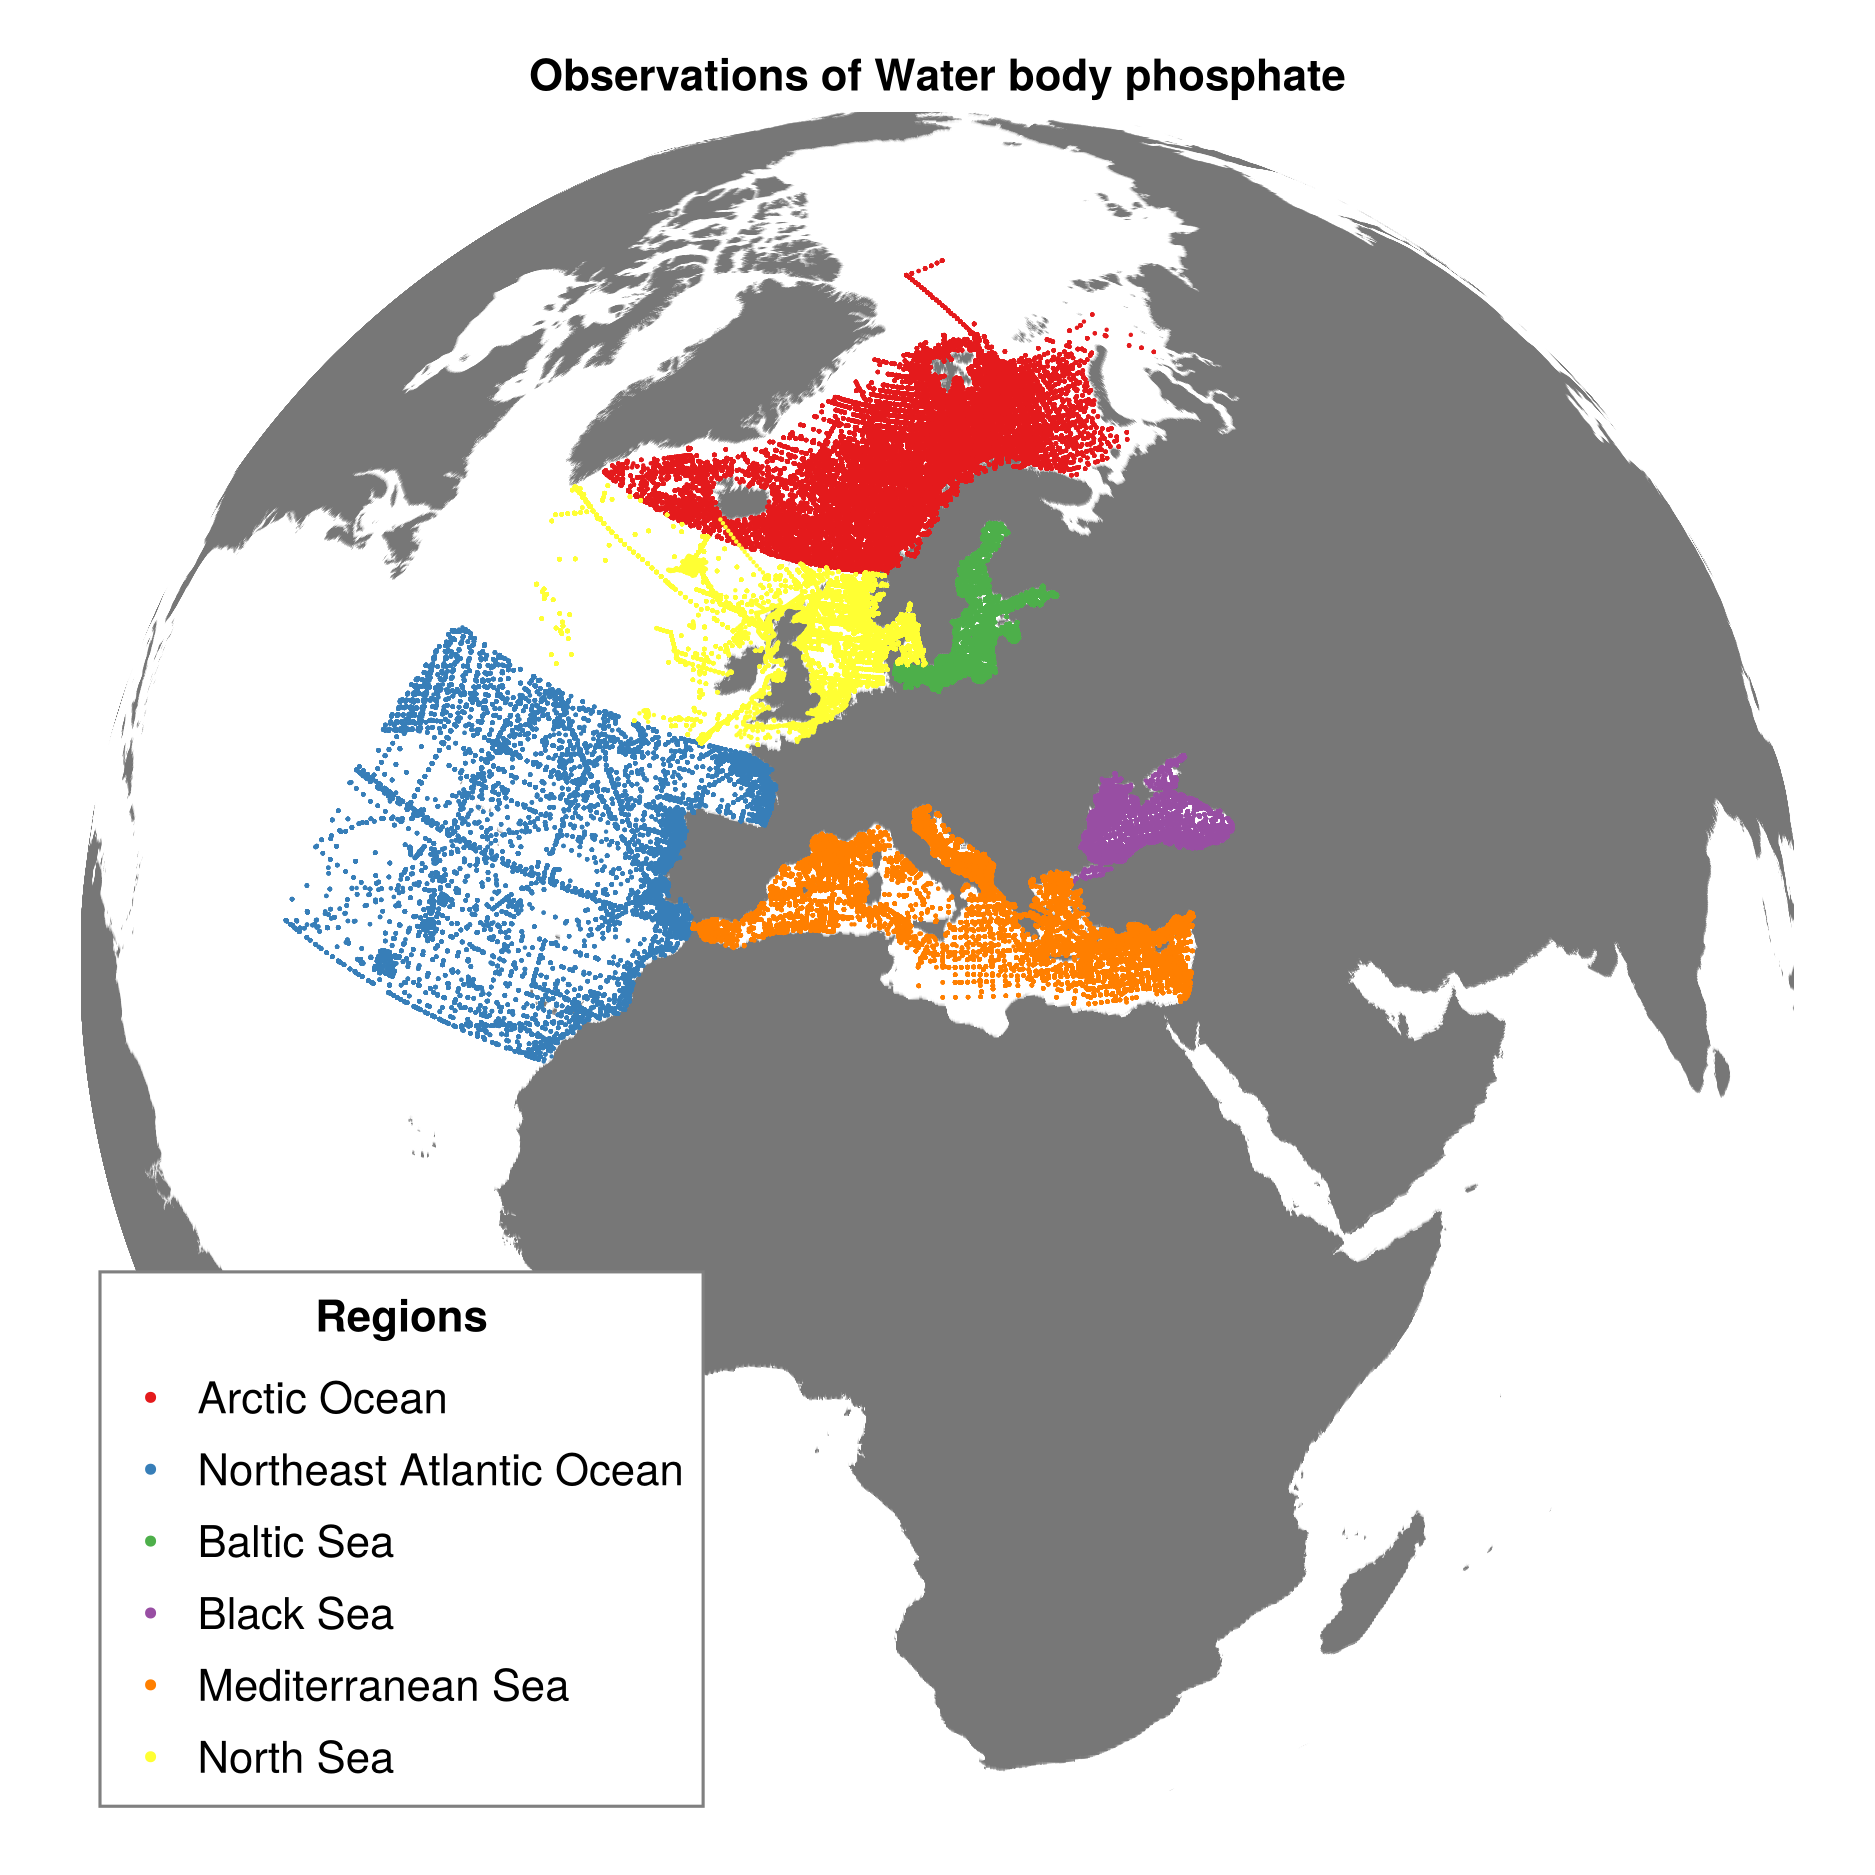
\includegraphics[width=8.3cm]{observations_Water_body_phosphate.png}
\caption{Data locations corresponding for the phosphate concentration measurements.\label{fig:phosphatedata}}
\end{figure}

\begin{figure}[t]
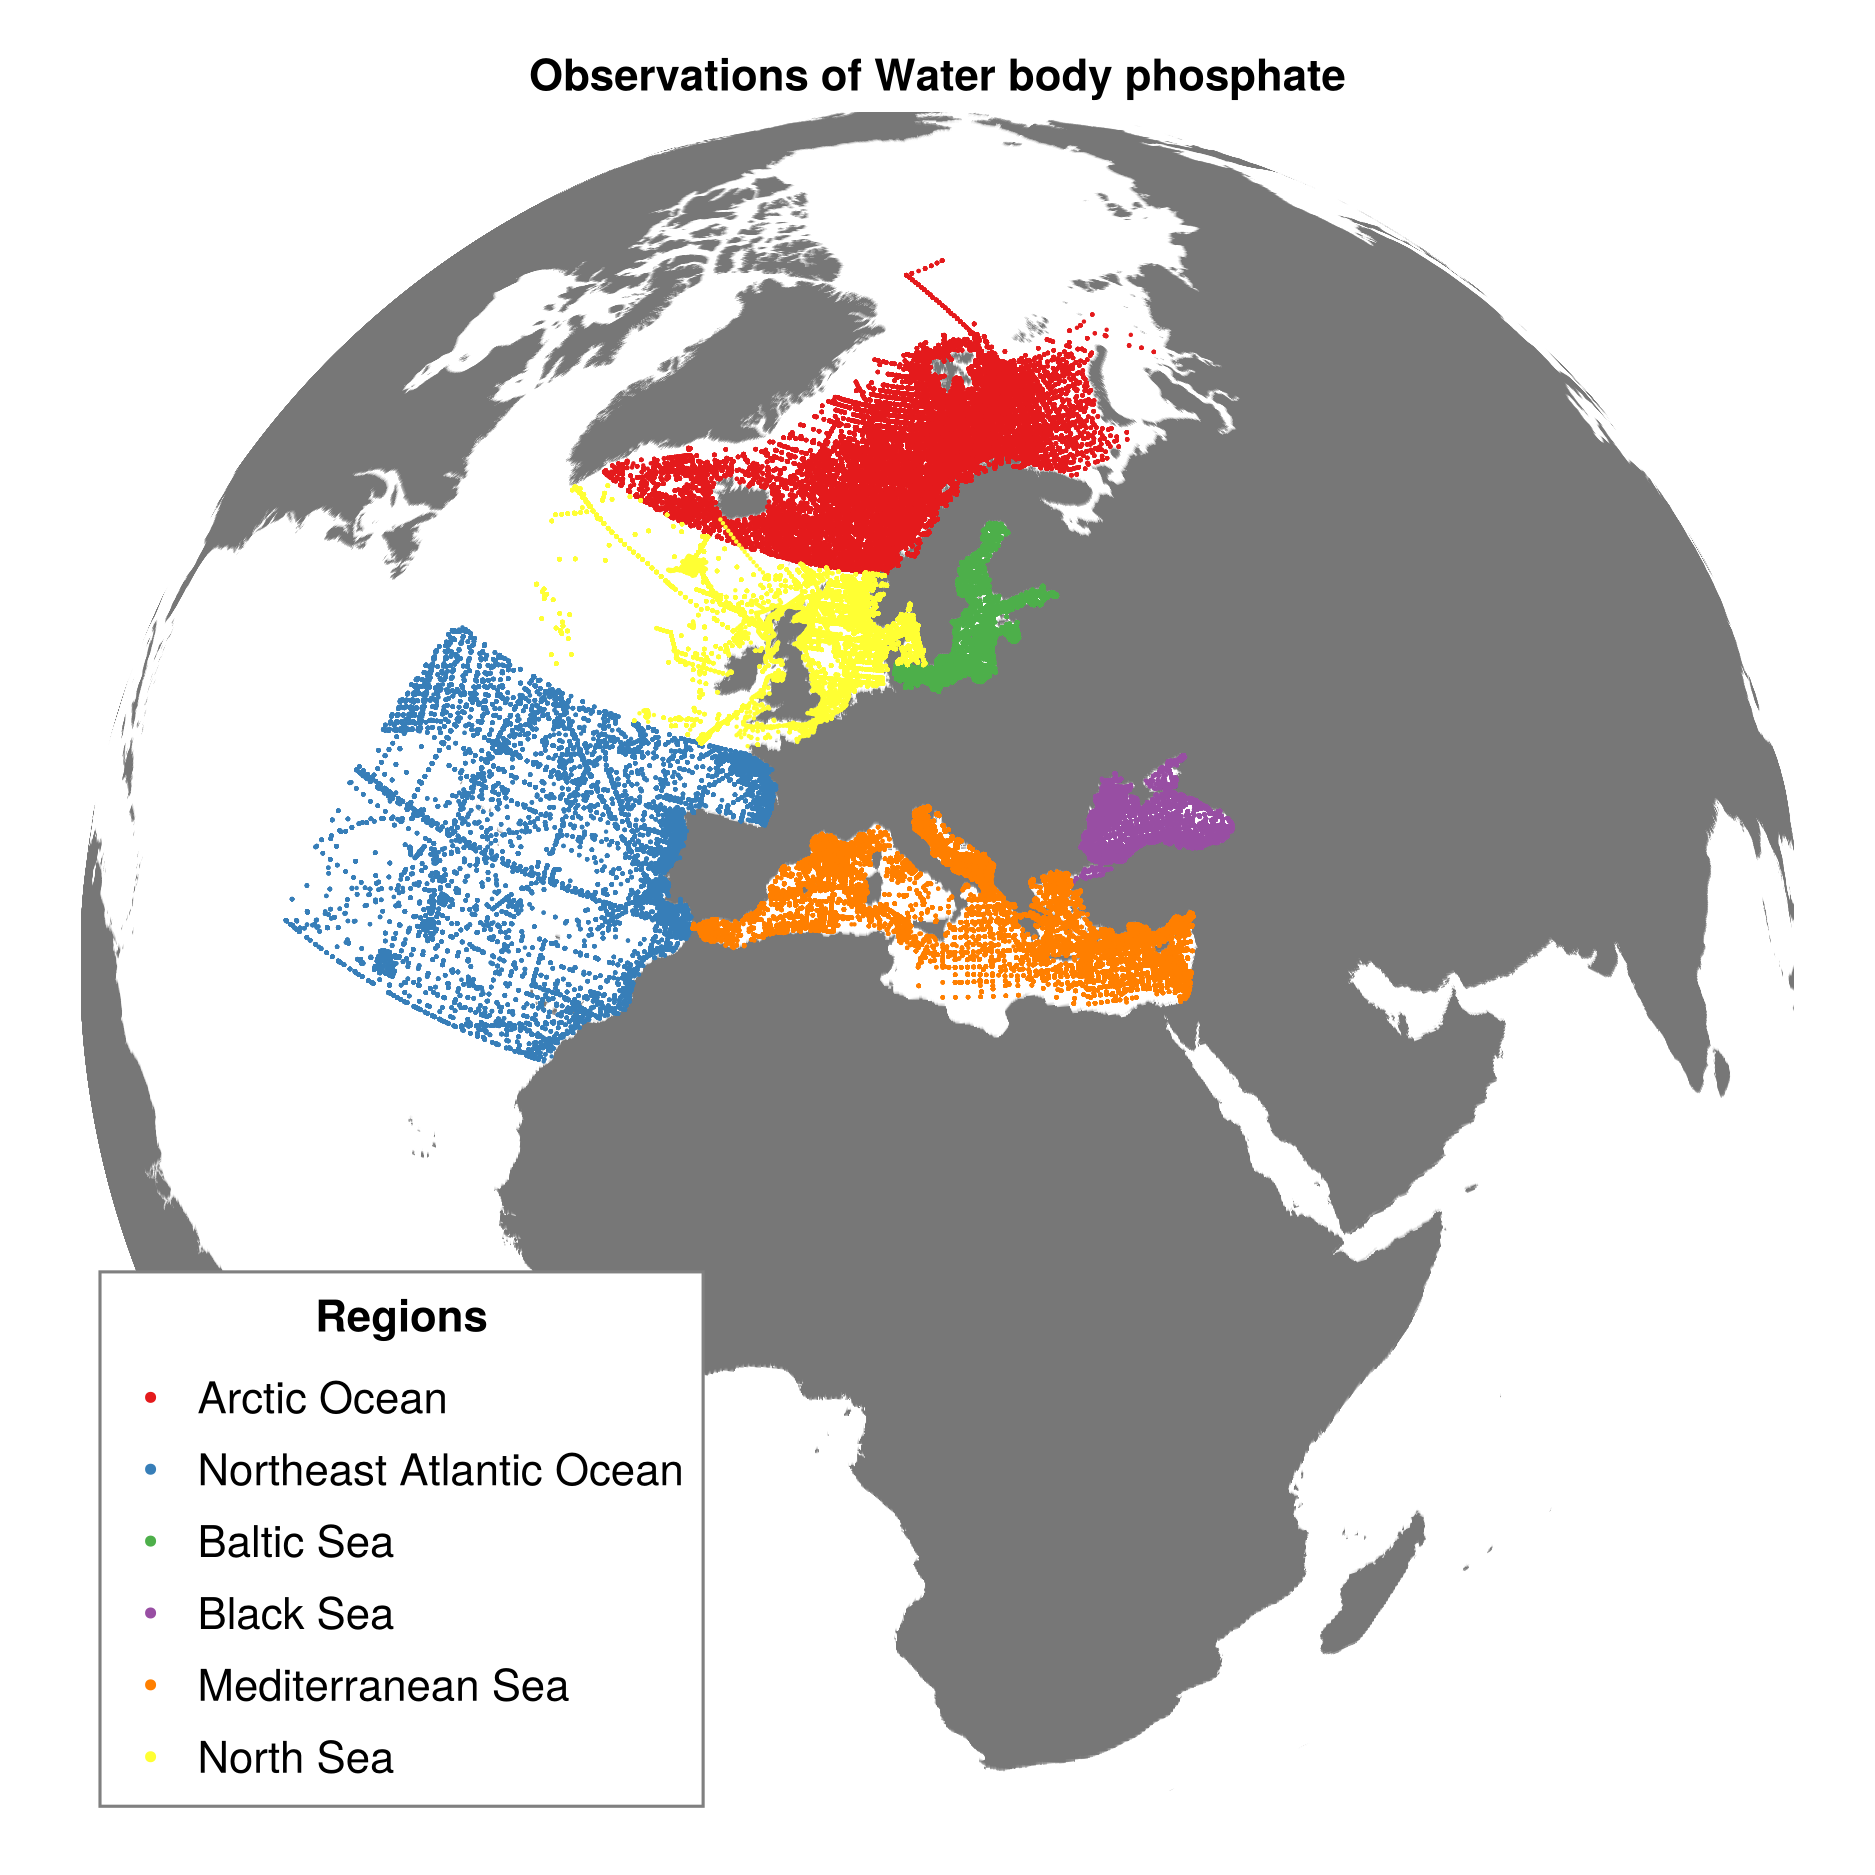
\includegraphics[width=8.3cm]{observations_Water_body_phosphate.png}
\caption{Data locations corresponding for the phosphate concentration measurements.\label{fig:phosphatedata}}
\end{figure}



\subsection{Domains}
The 6 regional domains are illustrated in Fig.~\ref{fig:phosphatedata} and were defined as follows:
\begin{description}
\item[Black Sea:] from 26.5°E to 41.95°E and from 40°N to 48°N;
\item[Mediterranean Sea:] from 6°W to 36.375°E and from 30°N to 46.375°N;
\item[Baltic Sea:] from 9.4°E to 30.9°E and from 53°N, to 66°N
\item[North Sea:] from 5.4°W to 13°E and from 48°N to 62°N;
\item[Arctic Sea:] from 42°W to 80°E and from 62°N to 83°N;
\item[North-East Atlantic Ocean:] from 42°W to 0° and from 24°N to 48°N.
\end{description}

		
The domains have been prepared so that there is no overlay between them, in particular: 
\begin{itemize}
\item The Mediterranean Sea and the Atlantic Ocean have their limit at the longitude of the Strait of Gibraltar;
\item The Sea of Marmara is assigned to the Mediterranean Sea region;
\item The North Sea and the NE Atlantic Ocean are separated by an imaginary line at 48°N, corresponding approximately to the latitude of Brittany (western France);
\item The Baltic Sea and the North Sea have their limit located 
\end{itemize}
We can see the almost straight lines corresponding to oceanographic campaigns and also the availability of coastal data, with the exception of the northern coast of Africa. 

\subsection{File preparation}

The original files are provided in the form of ODV \citep[Ocean Data View,][]{Schlitzer2002} collections. There are then converted to ODV netCDF, keeping the relevant metadata (i.e. those relative to the originators) in the exported files. Finally, the files are converted to ragged array netCDF using a script in Julia. The goal is to decrease the time needed to read the observations from the different regions: in the ODV netCDF files, the observations are organised by profile, and reading all of them means we have to loop over each profile. Meanwhile, for the creation of the gridded products, the information about the profile is not needed anymore and the data can be stored as vectors.

EDMO code and CDI \citep{Schaap2010}

With this format change, the files can be read in less than one minute (versus several hours for the ODV collections or ODV netCDF).

These operations were performed with ODV version 5.7.2 \citep{SCHLITZER2024}.
 

\subsection{Spatial distribution}

The hexbin plot (Fig. ) provides another view on the data density. The regions with the highest coverage are located in the Baltic Sea and in the southern part of the North Sean while in general lower data densities are found at the edges of the global domain. The Mediterranean sea also exhibits an inhomogeneous data coverage. 

The panels of Fig. x also highlights the differences between the variables: for phosphate, silicate and oxygen, most of the domain is covered, whereas for ammonium, dissolved organic nitrogen and, to a lesser extent, chlorophyll, large subdomains are almost void of measurements. This will impact the quality of the interpolated field (Section …), which depends on the quality of the measurements and their availability.











\subsection{Temporal distribution}
TEXT

\subsection{Value distributions}

The value distribution (Fig. ) shows different patterns according to the variable considered. The dissolved oxygen concentration is the closest to a Gaussian. Ammonium, chlorophyll-a, nitrogen and silicate distributions are all characterised by a dominant number of measurements for small concentrations (close to zero) and few observations of high concentration. The case of phosphate seems to be a superposition of the two previous cases, where the lar







\subsection{File format}
The original data collections are provided as ODV \citep[Ocean Data View,][]{SCHLITZER02} data collections. Such collections are easily read then exported to another format using the ODV software tool. In the present work we exported the collections to netCDF files, which are in turn are used as input files for the preparation of the climatologies (next Section). 
Along with the data (coordinates, time, depth and observed values), a set of metadata is assigned to each measurement. The complete list of metadata items is provided in the Appendix. Among them we find information about the instrument, the cruise and the institute that performed the measurements. 

\section{The interpolation method}

In this paper, we refer to \textit{gridding} as the process of computing the values of a variable (for instance: sea water temperature) on the nodes of a regular grid, based on observations of that variable at different locations and times.
The creation of gridded fields using sparse, in situ observations can be performed using different techniques. For the sake of simplicity, we will not review all of them but will insist on the distintion between two groups of tecniques:
\begin{enumerate}
\item The interpolation techniques: the field has to contain (or pass through) all the data points. For two-dimensional cases, an example of such a method is the bi-linear interpolation. Due to the different types of noise affecting the measurements in the ocean (instrumental, representativity, \ldots), such techniques are not the most suitable.
\item The approximation 
\end{enumerate}

The climatologies, consisting of a set of gridded fields for different depths and time periods, are produced by applying the Data Interpolating Variational Analysis in n dimensions (DIVAnd, see next Section) to the datasets presented in Section~\ref{sec:insitu}. Such gridded fields are frequently used in oceanography, for different purposes ranging from data visualisation to model initialisation or validation of measurements.  
While temperature and salinity (T and S) climatologies have been produced for various regions of the World Ocean using different interpolation techniques, climatologies for eutrophication-related variables are less frequent. The World Ocean Atlas (WOA) makes climatologies available for oxygen \citep[Dissolved Oxygen, Apparent Oxygen Utilization, and Oxygen Saturation][]{Garcia2024} and for dissolved inorganic nutrients \citep[phosphate, nitrate and nitrate+nitrite, silicate][]{Garcia2024b} at a resolution of 1° by 1° for the global ocean. The availability of measurements from the EMODnet Chemistry data collections makes it  possible to increase the spatial resolution in certain domains, hence the interest of the regional products presented in this paper.

% Check this → https://briochemc.github.io/WorldOceanAtlasTools.jl/stable/

\subsection{Method}

DIVAnd is an analysis method designed to generate fields on a curvilinear grid grid from a set of in situ measurements \citep{BARTH2014}. It is a new version of the DIVA tool (REFERENCES) that was previously limited to 2 dimensions (usually longitude and latitude). With DIVAnd, it is now possible to perform the analysis on an arbitrary number of dimensions, typically the horizontal dimension (longitudes and latitudes), the vertical dimension (depth or pressure) and the time. With the previous version of  the DIVA tool, climatologies were obtained by stacking 2-dimensional layers computed for different depths and time periods. 
One of the main advantages of the method over widely used methods such as the Optimal Interpolation (OI, REFERENCE) is that DIVAnd (and DIVA) naturally takes into account physical obstacles, typically the presence of land separating two bodies of water.  
DIVAnd is written in Julia \citep{Bezanson2017}, a fast, dynamically-type programming language, designed to ensure high-performance computation. While the previous code was written in Fortran, Julia ensures that high-resolution analysis using several millions of data points could be run in reasonable times, i.e. maximum a few days for the largest domain. This is necessary as usually to create a regional climatology, it is necessary to repeat the analysis several times in order to adapt the parameters and possibly remove suspect observations.




\section{Gridded climatologies\label{sec:clim}}


\subsection{Product descriptions}

\subsubsection{File format}

The output of the analysis is a set of netCDF files storing the gridded fields generated by the analysis are written in netCDF \citep{Rew1990,Brown1993}, making use of the NCDatasets.jl library \citep{Barth2024}.


\conclusions  %% \conclusions[modified heading if necessary]
TEXT

\codedataavailability{The DIVAnd code, written in Julia language, is available from \url{https://github.com/gher-uliege/DIVAnd.jl}, under the GNU General Public License v2.0.
The merged data sets are provided at …, while the griddied fields are made available from the Sextant Catalog (\url{https://sextant.ifremer.fr/eng}).}





\authorcontribution{CT prepared the manuscript. ME and EQ coordinated the management of metadata (catalog and DOI). AB and CT: prepare the pan-European sea products; SI and MT: Mediterranean Sea. K.W. Baltic Sea; MML and JKR: North Sea; LB and GS: Black Sea; AKO: Arctic Sea; JG and NP: North Atlantic Ocean.} 

\competinginterests{The authors declare that there is no competing interest.}
\disclaimer{The data coverage obtained with the in situ measurements is heterogeneous, leading in higher uncertainties in the gridded field. The information contained in the gridded field believed to be trustworthy. However its accuracy and completeness cannot be guaranteed.  Whilst every effort has been made to ensure its reliability within the limits of present knowledge, no responsibility can be accepted by those involved in its compilation or publication for any consequential loss or damage arising from its use.
} 
\begin{acknowledgements}
The European Marine Observation and Data Network (EMODnet) is financed by the European Union under Regulation (EU) No 508/2014 of the European Parliament and of the Council of 15 May 2014 on the European Maritime and Fisheries Fund. Part of the PHIDIAS project infrastructure (European Union’s Connecting Europe Facility under grant agreement No. INEA/CEF/ICT/ A2018/1810854) was used to run the pan-European Sea analysis.
\end{acknowledgements}

\bibliography{emodnet.bib}
\bibliographystyle{copernicus.bst}


% The figure files should be labelled correctly with Arabic numerals (e.g. fig01.jpg, fig02.png).


%% ONE-COLUMN FIGURES

%%f
%\begin{figure}[t]
%\includegraphics[width=8.3cm]{FILE NAME}
%\caption{TEXT}
%\end{figure}
%
%%% TWO-COLUMN FIGURES
%
%%f
%\begin{figure*}[t]
%\includegraphics[width=12cm]{FILE NAME}
%\caption{TEXT}
%\end{figure*}
%
%
%%% TABLES
%%%
%%% The different columns must be seperated with a & command and should
%%% end with \\ to identify the column brake.
%
%%% ONE-COLUMN TABLE
%
%%t
%\begin{table}[t]
%\caption{TEXT}
%\begin{tabular}{column = lcr}
%\tophline
%
%\middlehline
%
%\bottomhline
%\end{tabular}
%\belowtable{} % Table Footnotes
%\end{table}
%
%%% TWO-COLUMN TABLE
%
%%t
%\begin{table*}[t]
%\caption{TEXT}
%\begin{tabular}{column = lcr}
%\tophline
%
%\middlehline
%
%\bottomhline
%\end{tabular}
%\belowtable{} % Table Footnotes
%\end{table*}
%
%%% LANDSCAPE TABLE
%
%%t
%\begin{sidewaystable*}[t]
%\caption{TEXT}
%\begin{tabular}{column = lcr}
%\tophline
%
%\middlehline
%
%\bottomhline
%\end{tabular}
%\belowtable{} % Table Footnotes
%\end{sidewaystable*}
%
%
%%% MATHEMATICAL EXPRESSIONS
%
%%% All papers typeset by Copernicus Publications follow the math typesetting regulations
%%% given by the IUPAC Green Book (IUPAC: Quantities, Units and Symbols in Physical Chemistry,
%%% 2nd Edn., Blackwell Science, available at: http://old.iupac.org/publications/books/gbook/green_book_2ed.pdf, 1993).
%%%
%%% Physical quantities/variables are typeset in italic font (t for time, T for Temperature)
%%% Indices which are not defined are typeset in italic font (x, y, z, a, b, c)
%%% Items/objects which are defined are typeset in roman font (Car A, Car B)
%%% Descriptions/specifications which are defined by itself are typeset in roman font (abs, rel, ref, tot, net, ice)
%%% Abbreviations from 2 letters are typeset in roman font (RH, LAI)
%%% Vectors are identified in bold italic font using \vec{x}
%%% Matrices are identified in bold roman font
%%% Multiplication signs are typeset using the LaTeX commands \times (for vector products, grids, and exponential notations) or \cdot
%%% The character * should not be applied as mutliplication sign
%
%
%%% PHYSICAL UNITS
%%%
%%% Please use \unit{} and apply the exponential notation


\end{document}



